\documentclass{beamer}
\usepackage[brazil]{babel}
\usepackage[T1]{fontenc}

% other packages
\usepackage{latexsym,amsmath,xcolor,multicol,booktabs}
\usepackage{graphicx,pstricks,listings,stackengine}

\author{Gabriel Massi de Moura, Nathan Trugilho Braga e Pedro Victor Ferreira}
\title{Banco de Dados de Multimídia}
\institute{CEFET-RJ}
\usepackage{LZJTU}

% defs
\def\cmd#1{\texttt{\color{red}\footnotesize $\backslash$#1}}
\def\env#1{\texttt{\color{blue}\footnotesize #1}}
\definecolor{deepblue}{rgb}{0,0,0.5}
\definecolor{deepred}{rgb}{0.6,0,0}
\definecolor{deepgreen}{rgb}{0,0.5,0}
\definecolor{halfgray}{gray}{0.55}

\lstset{
    basicstyle=\ttfamily\small,
    keywordstyle=\bfseries\color{deepblue},
    emphstyle=\ttfamily\color{deepred},    % Custom highlighting style
    stringstyle=\color{deepgreen},
    numbers=left,
    numberstyle=\small\color{halfgray},
    rulesepcolor=\color{red!20!green!20!blue!20},
    frame=shadowbox,
}

\begin{document}

\begin{frame}
    \titlepage
    \begin{figure}[htpb]
        \begin{center}
            
\includegraphics[width=0.2\linewidth]{pic/logo.PNG}
        \end{center}
    \end{figure}
\end{frame}

\begin{frame}
    \tableofcontents[sectionstyle=show,subsectionstyle=show/shaded/hide,subsubsectionstyle=show/shaded/hide]
\end{frame}


\section{Introdução}

    \begin{frame}{Bancos Multimídia}
        \begin{itemize}
           \item  Nos anos 1990, a demanda por manipulação de mídia aumentou consideravelmente.
            \item Os modelos relacionais utilizados na época não eram mais totalmente adequados para o gerenciamento dos dados multimídia.
            \item Desde os anos 2000, o cenário dos Bancos Multimídia vem evoluindo para adequar melhores formas de gerenciamento e melhores desempenhos.
        \end{itemize}
    \end{frame}

\section{Definição}
    
    \subsection{Diferenças}
    
    \begin{frame}{Diferença entre Dado Convencional e Dado Multimídia}
        \begin{itemize}
            \item Dado Convencional: Texto, Números (Unidimensional)
            \item Dado Multimídia: Elementos de mídia (Composto)
        \end{itemize}
    \end{frame}
    
    \subsection{Problemas}

        \begin{frame}{Problemas em um Bando de Dados Multimídia}
            \begin{itemize}
                \item Escolha do método de captura de conteúdo.
                \item Resultados de consulta complexos.
                \item Dados de tamanho considerável.
                \item Tempo de recuperação da informação.
            \end{itemize}
        \end{frame}
    
    \subsection{Tipos de Mídia}
    
    \begin{frame}{Tipos de Mídia}
        \begin{itemize}
            \item Mídia de Percepção
            \item Mídia de Representação
            \item Mídia de Apresentação
            \item Mídia de Armazenamento
            \item Mídia de Transmissão
        \end{itemize}
        
    \end{frame}
    
    \subsection{Formatos de Mídia}
    
    \begin{frame}{Formatos de Mídia}
        \begin{itemize}
                \item Texto
                \item Gráfico
                \item Animação
                \item Imagem
            \end{itemize}
    
    \end{frame}

\section{Arquitetura}
        \begin{frame}{Arquitetura}

            \begin{figure}[htpb]
                \begin{center}
                    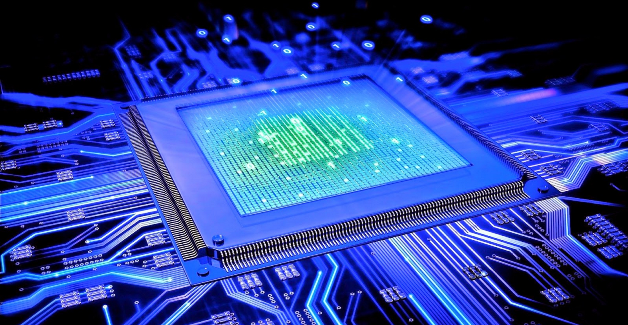
\includegraphics[width=0.8\linewidth]{pic/Arquitetura1.png}
                \end{center}
            \end{figure}
            
        
        \end{frame}
    
    \subsection{Os modelos possíveis}
        \begin{frame}{Arquitetura}
                
            Um modelo possível é o do  [De Biazi and Hoffmann Filho ]  que propõe três formas distintas de organização para bancos de dados multimídia, com base nos princípios de autonomia, uniformidade ou organização híbrida.
            
        \end{frame}
    \subsection{Princípio da Autonomia}
        \begin{frame}{Autonomia}
                
            \begin{figure}[htpb]
                \begin{center}
                    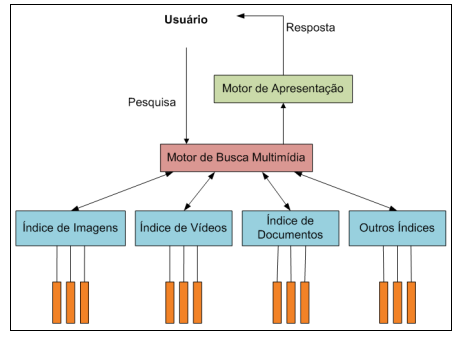
\includegraphics[width=0.8\linewidth]{pic/Autonomia.png}
                \end{center}
            \end{figure}
            
        \end{frame}
        
    \subsection{Princípio da Uniformidade }
        \begin{frame}{Uniformidade} 
                
            \begin{figure}[htpb]
                \begin{center}
                    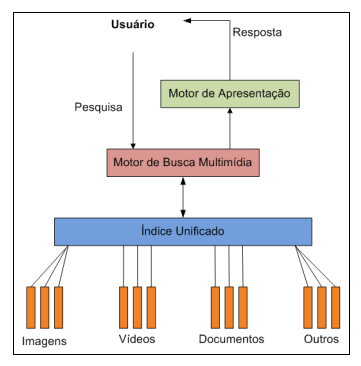
\includegraphics[width=0.5\linewidth]{pic/Uniformidade.png}
                \end{center}
            \end{figure}
            
        \end{frame}
        
    \subsection{Princípio Híbrido}
        \begin{frame}{Híbrido}
                
            \begin{figure}[htpb]
                \begin{center}
                    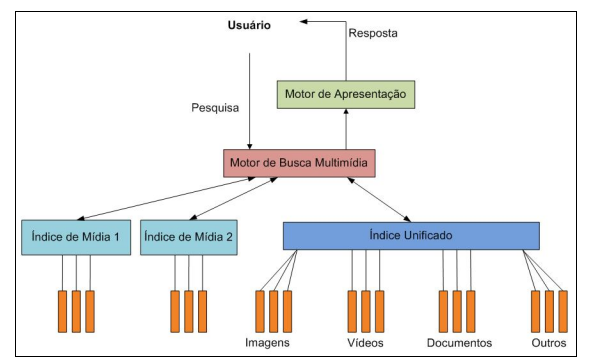
\includegraphics[width=0.8\linewidth]{pic/Híbrido.png}
                \end{center}
            \end{figure}
            
        \end{frame}
    
        

    
\section{SGBD Multimídia}
    
    \subsection{Características}
        \begin{frame}{O que é:}
        
        O SGBD multimídia pode ser compreendido como o conjunto de processos empregados
        para definir, criar, armazenar, indexar, gerenciar e pesquisar em bancos de dados multimídia.
        
        \end{frame}
        
        \begin{frame}{Características:}

        \begin{itemize}
            \item Integração de Dados 
            \pause \item Independência de Dados
            \pause \item Controle de Concorrência
            \pause \item Persistência
            \pause \item Controle de acesso
            \pause \item Controle de integridade
            \pause \item Recuperação
            \pause \item Processamento de pesquisa
            \pause \item Controle de versão.
            \end{itemize}
        \end{frame}

    \subsection{Requisitos}
    
        \begin{frame}{Características de um SGBDMM:}

        \begin{itemize}
            \item Métodos de indexação, pesquisa e organização dos dados multimídia
            \item Linguagens formais de pesquisa em ambiente multimídia
             \item Sincronização e integração de diferentes tipos de dados multimídia
            \item Estruturas eficientes de armazenamento de dados
            \item Integração e suporte ao sistema operacional
            \item Gerenciamento de bancos de dados multimídia distribuídos
            \item Técnicas de modelagem formais para dados multimídia
            \end{itemize}
        \end{frame}
        
        \begin{frame}{Características dos dados multimídia:}

        \begin{itemize}
            \item A estrutura detalhada dos objetos multimídia;
            \item As operações pertinentes aos objetos multimídia; 
            \item As propriedades dos objetos multimídia;
            \item Os relacionamentos entre os objetos multimídia e os objetos do mundo real;
            \item Propriedades, relacionamentos e operações em objetos do mundo real.
            \end{itemize}
        \end{frame}
        
\section{Armazenamento}
    \subsection{Referências externas}
        \begin{frame}{Referências externas}
            \begin{itemize}
                \item O banco de dados não tem controle direto sobre o objeto multimídia, pois este é armazenado fora do banco de dados, que mantém apenas uma referência ao local do objeto.
               \pause \item Pode causar \textcolor{red}{inconsistências} \pause $\rightarrow$ Pode referenciar um objeto inexistente. 
               \pause \item Viabiliza um \textcolor{blue}{acesso em tempo real} ao objeto multimídia.
               \pause \item Evita o carregamento desnecessário de grandes volumes de dados.
            \end{itemize}
        \end{frame}

    \subsection{Dados multimídia não interpretados}
        \begin{frame}{Dados multimídia não interpretados}
            \begin{itemize}
                \item Utiliza campos do banco de dados para armazenar dados brutos de multimídia, esses dados são armazenados como tipos de dados binários, os BLOBs (Binary Large Objects).
                \pause \item \textcolor{red}{Ocupa muito espaço do banco de dados}, o que afeta o desempenho em cenários de leitura intensiva.
                \pause \item O acesso a dados multimídia é \textcolor{blue}{rápido}, porque não há necessidade de realizar operações de entrada e saída.
                \pause \item A recuperação de dados é simples.
            \end{itemize}
        \end{frame}

    \subsection{Funções externas}
        \begin{frame}{Funções Externas}
            \begin{itemize}
                \item Pela limitação de recursos para manipular dados multimídia nos SGBDs, usa-se funções externas ao banco de dados.
                \pause \item As funções externas são criadas fora do banco de dados e podem ser implementadas em diversas linguagens como C, Java, Python entre outras.
                \pause \item Permite a utilização de bibliotecas especializadas fora do ambiente de banco do dados.
                \pause \item Pode ser difícil garantir a segurança e a integridade dos dados.
            \end{itemize}
        \end{frame}

    \subsection{Orientação a objetos}
        \begin{frame}{Orientação a objetos}
            \begin{itemize}
                \item Nos sistemas orientados a objeto, é possível definir tipos de dados e referenciá-los na aplicação.
                \pause \item Modelagem próxima ao domínio do problema, facilitando a compreensão e manutenção do código.
                \pause \item Persistem desafios relacionados à gestão \textcolor{red}{deficiente} do acesso em tempo real.
                \pause \item Método de armazenamento mais apropriado.
            \end{itemize}
        \end{frame}

    \subsection{Comparativo entre as formas de armazenamento}
        \begin{frame}{Comparativo entre as formas de armazenamento}
            \begin{figure}[htpb]
                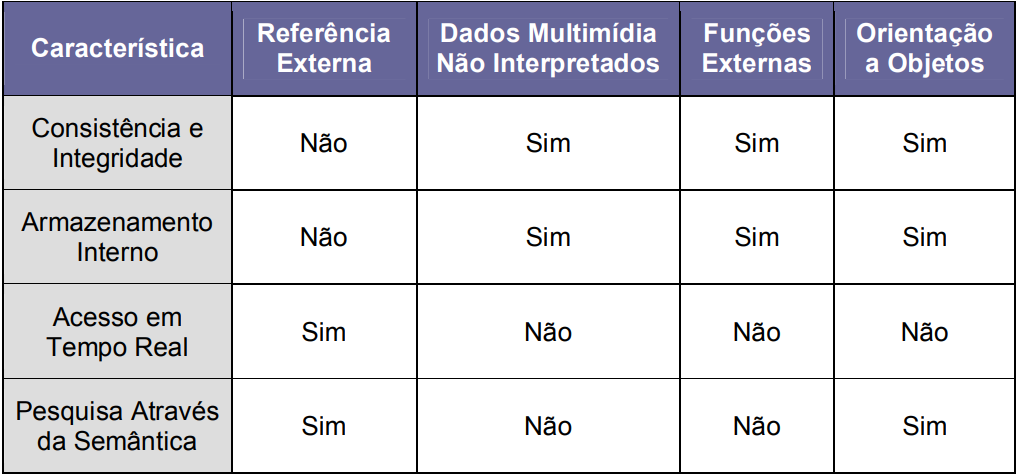
\includegraphics[width=1\linewidth]{pic/image.jpg}
            \end{figure}
        \end{frame}
    
\section{Aplicações}
    \begin{frame}{Aplicações de banco de dados de multimídia}
        \begin{itemize}
            \item \textbf{Gerenciamento de documentos e registros}
            \item \textbf{Disseminação de conhecimento}
            \item \textbf{Educação e treinamento}
            \item \textbf{Marketing, propagandas, vendas no varejo, entretenimento e turismo}
            \item \textbf{Controle e monitoramento em tempo real}
        \end{itemize}
    \end{frame}

\begin{frame}{Referências}
    
    De Biazi, D. and Hoffmann Filho, L. J. Banco de dados multimídia.
    \addlinespace
    \addlinespace
    Silva, R. C. (2006). Benchmark em Banco de Dados Multimídia: Análise de Desempenho em Recuperação de Objetos Multimídia. PhD thesis, Dissertação de Mestrado,
    Universidade Federal do Paraná, Curitiba.

\end{frame}

\begin{frame}
   \begin{figure}[htpb]
        \begin{center}
            
\includegraphics[width=0.6\linewidth]{pic/folkss.PNG}
        \end{center}
    \end{figure}
\end{frame}

\end{document}
